
\subsection{Correlation Analysis}
\label{app:correlation_analysis}
As the current language models are all exposed to Wikipedia knowledge during training, we are interested in how the LLM performance is correlated with the attributes of the triples in the knowledge graphs. As an example, if an entity has a higher degree, it may be linked to more documents, and the LLM may have more chances to learn about the entity during training. Another example is the popularity of the entity. If the entity is more popular, it may be linked to more external documents \wfj{because it summarizes the relevant knowledge and provides high-level ideas to the general public}, and the LLM may have more chances to learn about the entity during training. This raises the question of whether the LLM's performance is correlated with the attributes of the triples in the knowledge graphs.
For the entities in a knowledge graph, the degree of an entity is the number of edges connected to the entity. We also collect the \textit{pageviews} of the entities in the knowledge graph from Wikimedia\footnote{https://wikimedia.org/api/rest\_v1/metrics/pageviews/per-article/en.wikipedia.org/all-access/all-agents}{}, which is the number of pageviews of the Wikipedia page of the entity. This can be seen as a measure of the popularity of the entity  \wfj{because a popular page should appeal to the significant attention of the readers}. We collect the pageviews, in the time period of the entities in the knowledge graph from the Wikipedia page of the entity.
After collecting the degree and pageviews of the entities in the knowledge graph, we can aggregate the degree and pageviews of the entities to the triples, by simply taking the average of the degree and pageviews of the head and tail entities of the triples.

Here, we analyze whether the LLM's performance is correlated with the attributes of the triples in the knowledge graphs, such as the entity's degree, and page views. 
We refer to Figure \ref{fig:correlation_heatmap} for the correlation heatmap of the LLMs' hidden states and the judge model's predictions. Here, `T' stands for \textit{Truthful}, `I' stands for \textit{Informativeness}, `C' stands for \textit{Correctness}, `P' stands for Pageviews, and `D' stands for Degree. 
 We can see that the LLM's performance does not show a strong correlation with the attributes of the triples in the knowledge graphs. This indicates that the LLM's performance is not directly correlated with the attributes of the triples in the knowledge graphs. However, the different metrics of LLMs may correlate with each other, such as \textit{Truthful} and \textit{Informativeness}, which is expected. 
\xzrevision{This can be explained by the fact that certain attributes, like the degree of an entity in the knowledge graph, can be misleading. For example, degree is often correlated with popularity, but the popularity metric is 0 for many entities, particularly those in the long tail. This uneven distribution limits the usefulness of popularity as a reliable metric for evaluating LLM performance. In other words, while high-degree or popular entities may influence LLM performance to some extent, the vast majority of entities are long-tail, and their sparse or zero popularity values do not strongly correlate with performance outcomes. This highlights the need for more nuanced or domain-specific metrics to assess LLM performance effectively.}

\begin{figure}[t]
\centering
\subfloat[LLaMA-2-7B]{
 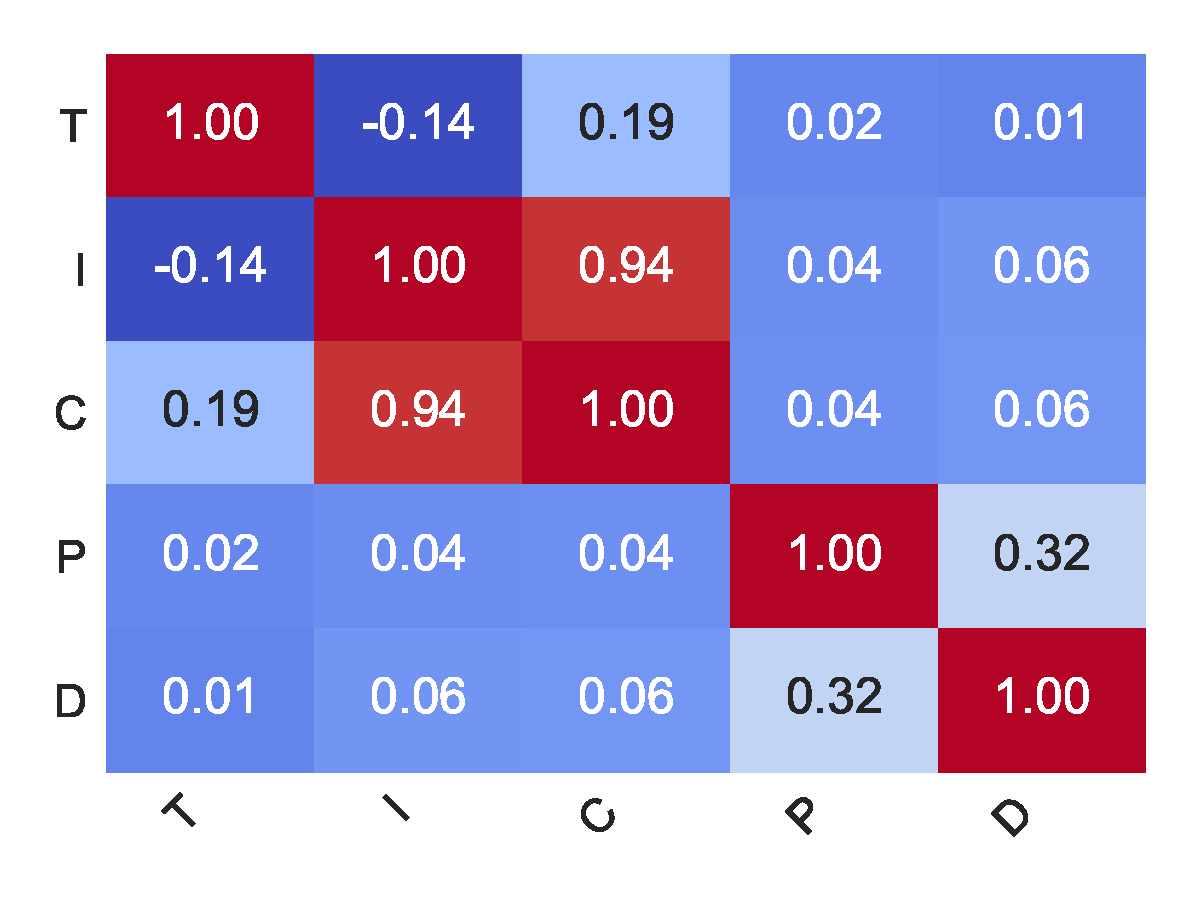
\includegraphics[width=1.6in]{submissions/Jing2024/figures/experiments/correlation_heatmap/correlation_heatmap_llama_7b.pdf}
 \label{fig:correlation_heatmap_llama_7b}
} 
\subfloat[LLaMA-2-13B]{
 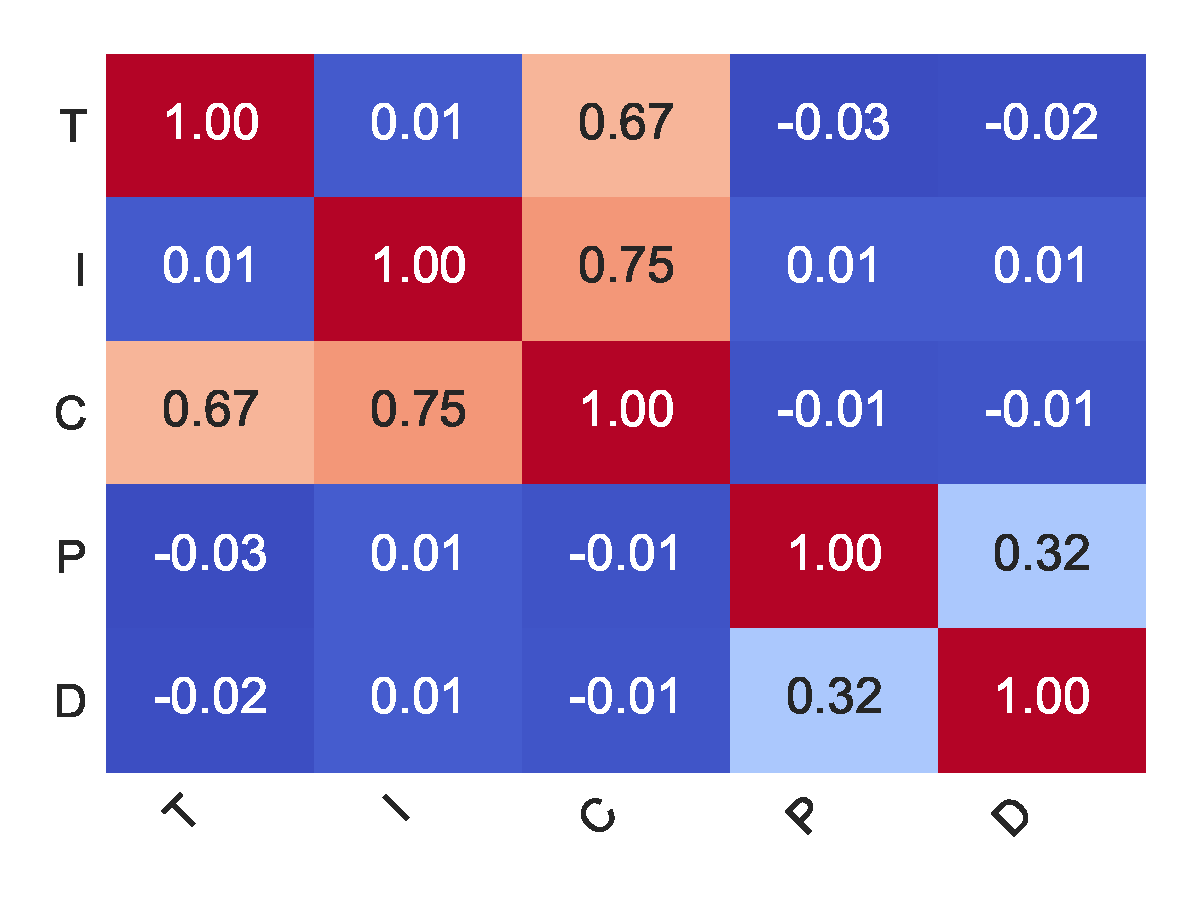
\includegraphics[width=1.6in]{submissions/Jing2024/figures/experiments/correlation_heatmap/correlation_heatmap_llama_13b.pdf}
 \label{fig:correlation_heatmap_llama_13b}
} 
\subfloat[LLaMA-2-70B]{
 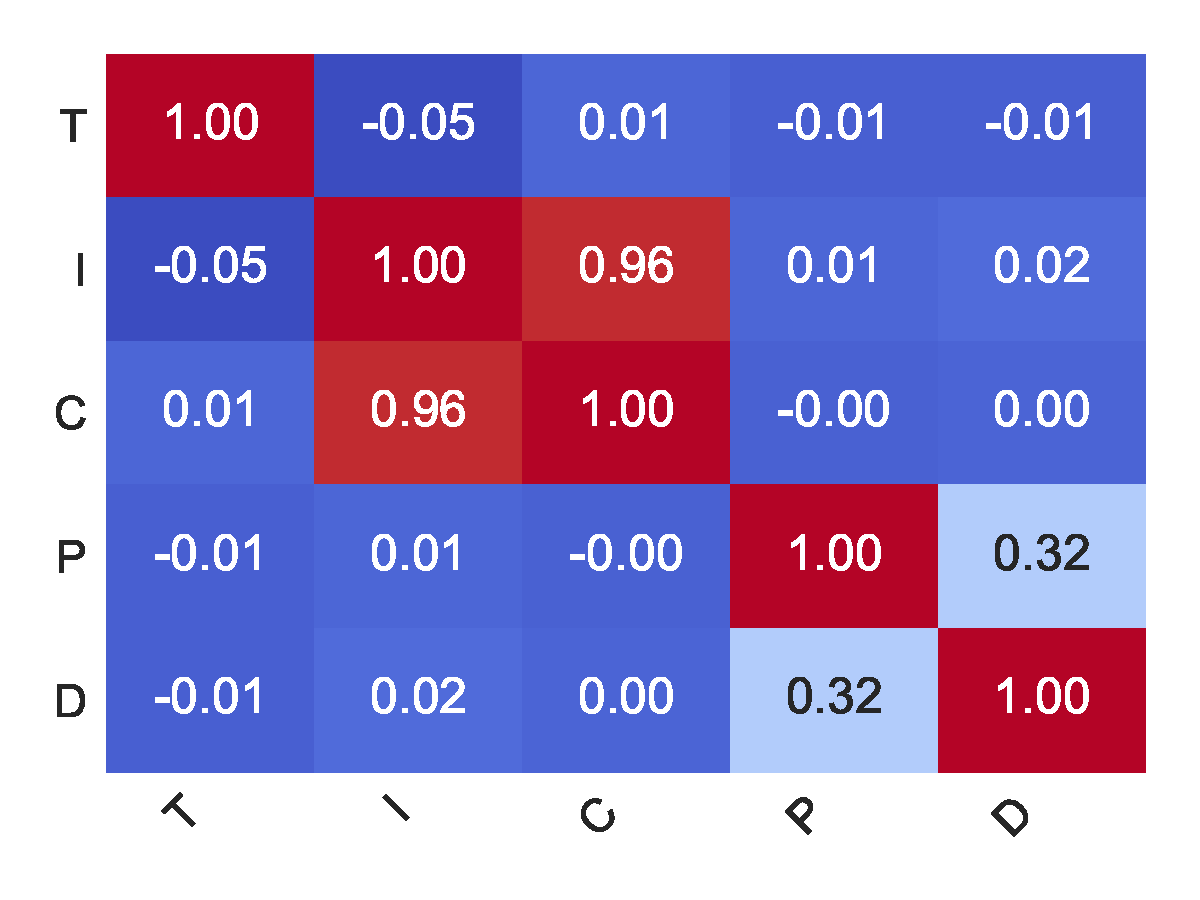
\includegraphics[width=1.6in]{submissions/Jing2024/figures/experiments/correlation_heatmap/correlation_heatmap_llama_70b.pdf}
 \label{fig:correlation_heatmap_llama_70b}
}
\\
\subfloat[Gemma-2B]{
 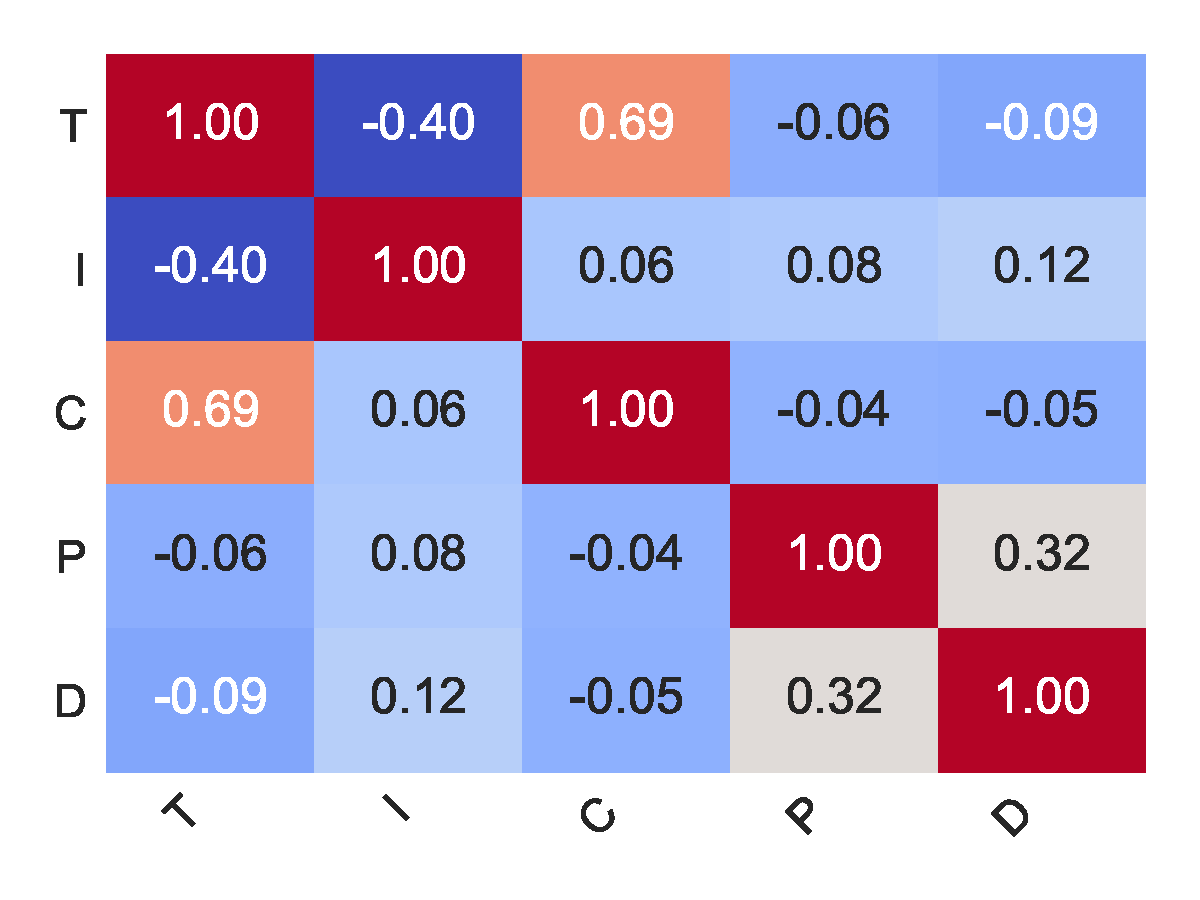
\includegraphics[width=1.7in]{submissions/Jing2024/figures/experiments/correlation_heatmap/correlation_heatmap_gemma_2b.pdf}
 \label{fig:correlation_heatmap_gemma_2b}
}
\subfloat[Gemma-7B]{
 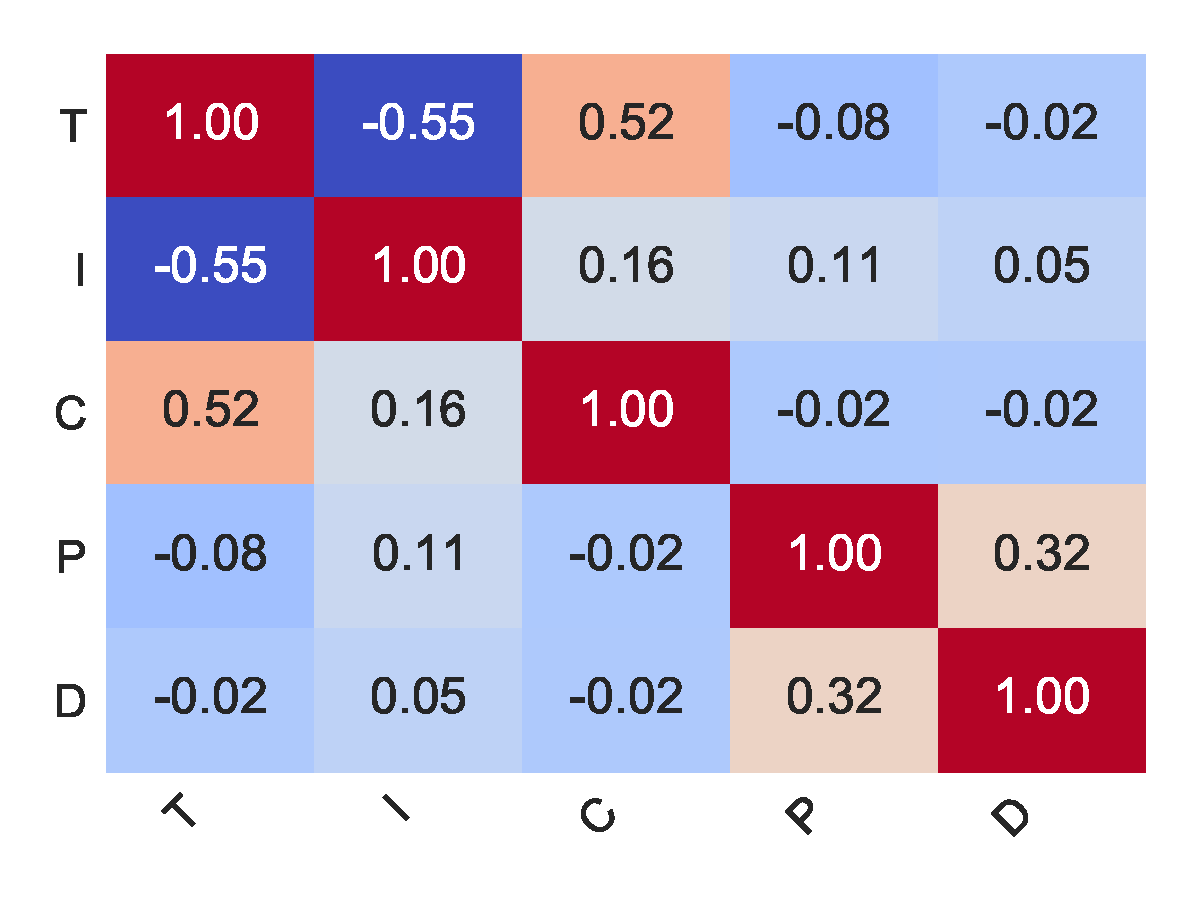
\includegraphics[width=1.7in]{submissions/Jing2024/figures/experiments/correlation_heatmap/correlation_heatmap_gemma_7b.pdf}
 \label{fig:correlation_heatmap_gemma_7b}
}
\caption{Correlation heatmap of the LLMs' hidden states and the judge model's predictions.}
\label{fig:correlation_heatmap}
\end{figure}


